\section{Introduction}
\begin{quote}
    \citep{pml1Book} -- Chapter 1.
\end{quote}

\subsection{Supervise Learning}
\textbf{Probabilistic perspective} ML: treat all unknown quantities as r.v.s.
endowed probability distribution describing a weighted set of the possible values.

\begin{note}
    Why is the probabilistic perspective adopted?
    \begin{enumerate}
        \item decision making under uncertainty and
        \item general language by other fields of science and engineering.
    \end{enumerate}
\end{note}


\textbf{Empirical risk} is the function of parameters $\bm{\theta}$, 
where the term \textit{empirical} implies using sample average to substitute population-level expectation 
(real data distribution is usually unknown), 
and the loss function $\ell(\cdot)$ can be specified according to real-world condition.
The model fitting is to find a \underline{minimizer} $\hat{\bm{\theta}}$ of $\mathcal{L}(\bm{\theta})$.
\begin{gather}
    \mathcal{L}(\bm{\theta})=\frac{1}{N}\sum_{n=1}^N
    {\ell(y_n,f(\bm{x}_n;\bm{\theta}))}
\end{gather}

\textbf{Conditional probability distribution} is adopted to capture the uncertainty.
\begin{gather}
    p(y|\bm{x};\bm{\theta})
    =f_y(\bm{x};\bm{\theta}):\mathcal{X}\to\mathcal{Y}
\end{gather}

\textbf{Deep neural networks} (vs linear\&polynomial regression) do 
nonlinear feature extraction automatically with stacked multiple hidden layers $\phi(\cdot;\bm{V})$
with $\bm{V}=[\bm{\theta}_1,\cdots,\bm{\theta}_{L-1}]$ 
and output the prediction with the final layer with $\bm{w}=\bm{\theta}_L$.
\begin{gather}
    f(\bm{x};\bm{w},\bm{V})=\bm{w}^T\phi(\bm{x};\bm{V})
\end{gather}

\begin{quote}\textit{
    Supervised learning is essentially just ``glorified curve fitting''.
}\end{quote}

\subsection{Unsupervised learning}

\textit{Unconditional} vs \textit{conditional}\unsure{
$\bm{y}$ follows mixed model with additional uncertainty of unknown co-variates
introduced by transformation from $\bm{x}$
}
models of \textit{unsupervised} vs \textit{supervised} learning.
\begin{gather}
    p(\bm{x})~\text{vs}~p(\bm{y}|\bm{x})
\end{gather}

% \begin{note}
    Strategies to find such model $p(\bm{x})$ generating data:
    \begin{enumerate}
        \item clustering by defining the similarity (distance in same space) among data points; 
        \item modeling the low-dimensional representation (Equation (\ref{eq:latent})) 
        of unobserved latent factors;
        \item self-supervised learning: 
        build proxy supervised tasks from unlabeled data, and 
        learn useful representation from the data themselves.
    \end{enumerate}
% \end{note}

\begin{example}
    \textbf{Modeling low-dimensional latent representation}\\
    \begin{gather}
        p(\bm{x}_n|\bm{z}_n;\bm{\theta})
        =N(\bm{x}_n|f(\bm{z}_n;\bm{\theta}),\bm{\Sigma})
        ~~~\bm{z}_n\in\mathbb{R}^K,~K\ll{D}
        \label{eq:latent}
    \end{gather}
    \begin{itemize}
        \item \textbf{Factor analysis}: 
        $f(\bm{z}_n;\bm{\theta})=\bm{W}\bm{z}_n+\bm{\mu}$
        \item \textbf{PCA}:
        $f(\bm{z}_n;\bm{\theta})=\bm{W}\bm{z}_n+\bm{\mu}$ and 
        $\bm{\Sigma}=\sigma^2\bm{I}$
        \item \textbf{Variational autoencoder}:
        $f(\cdot)$ neural network (nonlinear) and
        $\bm{\Sigma}=\sigma^2\bm{I}$
    \end{itemize}
\end{example}

Principles of evaluating unsupervised learning
\begin{enumerate}
    \item \textit{data compression as lossless as possible}:
    treat it as density estimation\unsure{
    recall the knowledge learned from \textit{Statistical Inference}}
    and see if a model captures the typical and useful patterns in the data;
    \item \textit{sample efficiency} of the learned representation: improvement in downstream application, 
    say, supervised learning tasks (easy to evaluate);
    \item \textit{interpretability}: discover the true underlying structure behind some dataset.
\end{enumerate}

\subsection{Reinforcement Learning}
\begin{figure}[htpb]
    \centering
    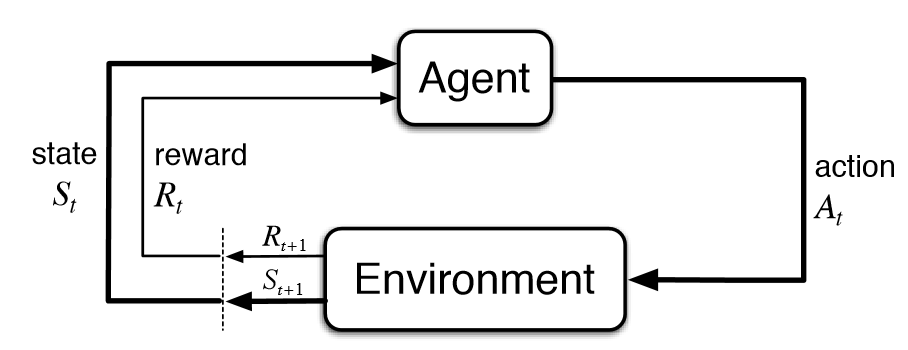
\includegraphics[width=0.7\textwidth]{figs/rl.png}
    \caption{Reinforcement Learning\protect\footnotemark[1]}
    \label{fig:rldiag}
\end{figure}
\footnotetext[1]{
\hyperlink{https://towardsdatascience.com/reinforcement-learning-101-e24b50e1d292}
{https://towardsdatascience.com/reinforcement-learning-101-e24b50e1d292}}

% \begin{quote}
%     Some key terms that describe the basic elements of an RL problem are\footnotemark[1]:
%     \begin{itemize}
%         \item Environment: Physical world in which the agent operates
%         \item State: Current situation of the agent
%         \item Reward: Feedback from the environment
%         \item Policy: Method to map agent’s state to actions
%         \item Value: Future reward that an agent would receive by taking an action in a particular state
%     \end{itemize}
% \end{quote}

Compared with supervised learning, the reward in RL may only be given occasionally and summarily
(e.g. if the agent eventually reaches a desired state after a path of actions)

\subsection{Data}

Common datasets (Benchmark):
\begin{itemize}
    \item small image datasets: MNIST [1,28,28] (extend to EMNIST, fashion-MNIST), CIFAR-10 [3,32,32];
    \item large image datasets: ImageNet [3,256,256];
    \item text datasets for text classification: IMDB movie review dataset;
    \item text datasets for machine translation: documents from multilingual organizations 
    (e.g. Canadian parliament and EU), WMT dataset;
    \item seq2seq tasks (e.g. document summarication and question answering): ?.
\end{itemize}

\textbf{TF-IDF}: term frequency-inverse document frequency.\unsure{
weighted BoW that reduce the importance of uninformative terms
}
TF$_{ij}$ is the frequency of term $i$ in document $j$, and 
IDF$_i\triangleq{\frac{N}{1+\text{DF}_i}}$, 
where $DF_i$ is the number of documents with term $i$.
\begin{gather}
    \text{TF-IDF}_{ij}=\log{\text{TF}_{ij}+1}\times\text{IDF}_i
\end{gather}

\textbf{Word embeddings}: 
\unsure{
Usually self-supervised models were adopted to build a pre-trained word embeddings 
based on large-scale contexts.
}\unsure{
The embeddings with similar meanings be often close in some metric space.}
map sparse and vocabulary-length (high-dimensional) vectors to 
dense and low-dimensional ones (embeddings).

Strategies to deal with OOV:
\begin{enumerate}
    \item replace all novel words with $\mathtt{UNK}$;
    \item byte-pair encoding: finer-grained subword structure embedding;
\end{enumerate}

Let $\bm{M}\in\mathbb{I}^{N\times{D}}$ indicates the missing status of feature $\bm{X}$:
$M_{nd}=1$ if $X_{nd}$ is missing and let $\bm{X}_v~(\bm{M}_v=\bm{0})$ and 
$\bm{X}_h~(\bm{M}_h=\bm{1})$ 
are visible and missing parts of features, respectively. 
The outcome labels $\mathbf{Y}$ are full observed.\unsure{
Missing data handling is a complex topic,
also important in \textit{clinical trial designing}, 
and will be discussed later and further.
}
\begin{itemize}
    \item \textbf{missing completely at random} (MCAR): 
    $p(\bm{M}|\bm{X}_v,\bm{X}_h,\bm{Y})=p(\bm{M})$,
    the missingness does not depend on the hidden/observed features;
    \item \textbf{missing at random} (MAR):
    $p(\bm{M}|\bm{X}_v,\bm{X}_h,\bm{Y})
    =p(\bm{M}|\bm{X}_v,\bm{Y})$,
    the missingness does not depend on the hidden features but may depend on the visible features;
    \item \textbf{not missing at random} (NMAR): otherwise
\end{itemize}

\begin{note}
    In the MCAR/MAR case, the missingness mechanism can be ignored since missingness is
    independent with the unobserved features. 
    And \textbf{this book always makes the MAR assumption}.
\end{note}

\section{Foundations}
\begin{quote}
    \citep{pml1Book} -- Chapter 2-8.
\end{quote}

\subsection{Probability: Univariable and Multivariable Models}

Types of uncertainty:
\begin{enumerate}
    \item \textbf{model uncertainty}: or epistemic uncertainty,
    caused by our ignorance of the underlying hidden causes or mechanism generating the data;
    \item \textbf{data uncertainty}: or aleatoric uncertainty,
    caused by intrinsic variability (the true model generating data randomly).
\end{enumerate}

Paradigm of binary classification with the assumption of probability output:
\begin{gather}
    p(y|\bm{x},\bm{\theta})
    =\text{Bernoulli}(y|\sigma(f(\bm{x};\bm{\theta})))
\end{gather}
where basic property of neuron, activation function $\sigma(a)$, in a network's output layer is compressing the value of unconstrained function to $[0,1]$, 
one example with good characteristics (refer to \citep{pml1Book} Table 2.3) 
of which is the sigmoid function $\frac{1}{1+e^{-a}}$, 
and the variety of $f$'s contributes to the contemporary blossom of deep learning architectures, 
the easiest one of which is linear model $\bm{w}^T\bm{x}+b$. (Logistic regression: Binomial+Sigmoid \& Multinomial+Softmax
\unsure{log-sum-exp trick for computer friendly to avoid floating-point overflow})

\textbf{Paradigm of regression}:
\begin{gather}
    p(y|\bm{x};\bm{\theta})
    =\mathcal{N}(y|
    f_\mu(\bm{x};\bm{\theta}),
    f_\sigma^2(\bm{x};\bm{\theta})
    )
\end{gather}
where $f_\mu\in\mathbb{R}$ predicts the mean 
and $f_\sigma^2\in\mathbb{R}^+$ predicts the variance.
Recall the two types of uncertainty,
the \textbf{uncertainty of data} ($y$) is presented by $f_\sigma(\bm{x};\bm{\hat{\theta}})$ and 
the \textbf{uncertainty of model} ($\bm{\theta}$) is presented by 
$\mathrm{Var}f_\mu(\bm{x};\bm{\theta})$.

Gaussian (or Normal) distribution has \textbf{good characteristics}
\begin{enumerate}
    \item with two parameters $\mu,\sigma^2$, easy to interpret;
    \item by central limit theorem (modeling the noise from multiple sources);
    \item with the least number of assumptions;
    \item with simple form, easy to implement but highly effective.
\end{enumerate}







